\section{Approach}
Given a video \(X_{0:T}\) with missing regions, STSENet targets to recover the complete video \(Y_{0:T}\), where $T$ is the total number of frames.
\( \widetilde{Y}_{0:T}\) is denoted as the ground truth video, and \(M_{0:T}\) is the mask sequence that indicates the missing regions in \(X_{0:T}\).
In each inference batch, to generate current frame \(Y_t\), total $5$ frames $\boldsymbol{X}$, indexed by (\(X_{t-7}, X_{t-3}, X_{t} ,X_{t+3}, X_{t+7}\)), are fed to STSENet, as well as corresponding mask $\boldsymbol{M}$.  
%$t$ is the index of the current frame.
%The ground truth video is \( \widetilde{Y}_{0:T}\). We use \(X_t\) to denote the \(t_{th}\) input frame, while the mask \(M_{0:T}\) indicates the missing region.
%The corresponding output video frame is \(Y_t\). To generate a precise \(Y_t\), we fed the network with neighbor frames $\boldsymbol{X}$, namely, (\(X_{t-7}, X_{t-3}, X_{t} ,X_{t+3}, X_{t+7}\)) and their corresponding masks $\boldsymbol{M}$, namely, (\(M_{t-7}, M_{t-3}, M_{t} ,M_{t+3}, M_{t+7}\)), which will help the network to borrow complementary information from different frames.
The intuition is that there exists complementary information in the neighbouring frames, which can benefit the inpainting process of the current frame.
As shown in Fig.~\ref{zong}, the architecture of our network is composed of three parts: a) an edge completion module that recovers spatial details of input frames; b) a flow completion module that completes motion between neighbor frames and target frame; and c) a frame inpainting module that generates spatio-temporal consistent frames with auxiliary inpainted edge and flow.
The detailed implementation of each part will be illustrated in the following sections.



%Our network is to recover the video \(Y_{0:T}\) from the incompleted video \(X_{0:T}\). The ground truth video is \( \widetilde{Y}_{0:T}\). We use \(X_t\) to denote the \(t_{th}\) input frame, while the mask \(M_t\) indicates the missing region. The corresponding output video frame is \(Y_t\). To generate a precise target frame \(Y_t\), we fed the network with neighbor frames $\boldsymbol{X}$, namely, (\(X_{t-7}, X_{t-3}, X_{t} ,X_{t+3}, X_{t+7}\)) and their corresponding masks $\boldsymbol{M}$, namely, (\(M_{t-7}, M_{t-3}, M_{t} ,M_{t+3}, M_{t+7}\)), which will help the network to borrow complementary information from different frames. The intuition is that there may exist relative information of the unseen part in current frame in other frames, which can aid the recovery process of the target frame.
%As shown in Fig.~\ref{zong}, the architecture of our network is composed of three parts, i.e., an edge completion module, a flow completion module, and a frame inpainting module. We will introduce details of each module in the following section. 



\subsection{Edge Inpainting Network}
Video inpainting suffers from the lack of structural details.
To generate an inpainting result with fine details, we first predict corresponding reasonable structural clues, which are beneficial to the following frame inpainting process.
%The edge completion module aims to generate the completed edge maps $\boldsymbol{E}$ for input frames $\boldsymbol{X}$. 

Given the incompleted grayscale images $\boldsymbol{X}^{g}$ of input frame, a canny edge detector is first used to generate initial edge maps $\boldsymbol{E}^{i}$. 
Then, an edge inpainting network (ENet) is designed to refine $\boldsymbol{E}^{i}$.
The input of ENet is a triplet of grayscale images, initial edge maps, and corresponding masks. 
The detailed implementation of ENet is shown in Fig.~\ref{enet}, which consists of a generator $N^E$ and a discriminator $D^E$.
$N^E$ contains a 2-layer 3D encoder, eight 2D residual blocks, and a 2-layer 3D decoder. The 3D encoder and decoder are designed to learn spatio-temporal information, while the 2D residual blocks are used to enrich the spatial features in a larger receptive field. The discriminator $D^E$ follows $70\times 70$ PatchGAN architecture \cite{Isola_2017_CVPR}.
Finally, the inpainted edge maps are obtained by:
\begin{equation}
\label{eq:edgenet}
\boldsymbol{E}=N^E(\boldsymbol{E}^{i},\boldsymbol{X}^{g},\boldsymbol{M}),
\end{equation}

The loss function for ENet is:
\begin{equation}
\label{eq:loss_e}
\mathcal{L}_{edge}=\mathcal{L}^E_{adv}+\lambda_1 * \mathcal{L}^E_{fm}
\end{equation}
where $\mathcal{L}^E_{adv}$ and $\mathcal{L}^E_{fm}$ are respectively the adversarial loss and feature matching loss. 
$\lambda_1$ is a hyper-parameter to balance different terms.
Following the adversarial learning manner, $\mathcal{L}^E_{adv}$ can facilitate ENet to produce realistic edge maps. The adversarial loss are defined by:
\begin{equation}
\label{eq:edge_adver}
\mathcal{L}^E_{adv}=\min\limits_{N^E} \max \limits_{D^E}\mathbb{E}[logD^E(\boldsymbol{E}^{gt},\boldsymbol{X}^{g})]+\mathbb{E}log[1-D^E(\boldsymbol{E},\boldsymbol{X}^{g})],
\end{equation}
where $E^{gt}$ represents the ground truth of edge maps 

$\mathcal{L}^E_{fm}$ evaluates the feature-level similarity between ground truth edge maps and predicted edge maps, which helps to create structurally rational edge maps. The feature matching loss is defined by:
\begin{equation}
\label{eq:edge_fm}
\mathcal{L}^E_{fm}=\sum_{k=1}^L{\frac{1}{N_k}\left\| D^E_k(\boldsymbol{E}^{gt},\boldsymbol{X}^{g})- D^E_k(\boldsymbol{E},\boldsymbol{X}^{g})\right\|_1},
\end{equation}
where $D^E_k$ denotes the $k$-th layer of $D^E$, while $N_k$ is the element number of the $k$-th layer.

\subsection{Optical Flow Completion Module}
It's important for video inpainting to maintain temporal consistency.
To this end, the optical flow completion module is designed to predict the motion tendency among frames.

Similar to ENet, the initial optical flow \(\boldsymbol{O}^i\) for $\boldsymbol{X}$ are first generated, using Flownet2.0 \cite{Flownet_2017_CVPR}.
Notably, \(\boldsymbol{O}^i\) consists of \((O^i_{t\Rightarrow t-7},O^i_{t\Rightarrow t-3},O^i_{t\Rightarrow t+3},O^i_{t\Rightarrow t+7})\).
Then, the proposed flow inpainting network (FNet) $N^F$ is used to refine \(\boldsymbol{O}^i\) by:
\begin{equation}
\label{eq:flownet}
\boldsymbol{O}=N^F(\boldsymbol{O}^{i},\boldsymbol{M}),
\end{equation}
where $\boldsymbol{O}$ is the refined optical flow.
FNet consists of ....
The detailed architecture of FNet is shown in Figure~\ref{enet}.

The loss function for FNet is :
\begin{equation}
\label{eq:flow_all}
\mathcal{L}_{flow}=\mathcal{L}^F_{rec}+\mathcal{L}^F_{har},
\end{equation}
where $\mathcal{L}^F_{rec}$ and $\mathcal{L}^F_{har}$ are respectively $l_1$-reconstruction loss and hard mining loss.
The $l_1$-reconstruction loss is defined as:
\begin{equation}
\label{eq:flow_l1}
\mathcal{L}^F_{rec}=\frac{1}{\left\|\boldsymbol{M} \right\|_1}\left\|(\boldsymbol{O}-\boldsymbol{O}^{gt})\odot \boldsymbol{M}\right\|_1,
\end{equation}
where $\boldsymbol{O}^{gt}$ is the ground truth. The symbol $\odot$ denotes the pixel-wise multiplication. Specifically, $\mathcal{L}^F_{rec}$ measures the difference between $\boldsymbol{O}^{gt}$ and $\boldsymbol{O}$.
The hard mining loss is defined as:
\begin{equation}
\label{eq:flow_hard}
\mathcal{L}^F_{har}=\frac{1}{\left\|\boldsymbol{M}_H \right\|_1}\left\|(\boldsymbol{O}-\boldsymbol{O}^{gt})\odot \boldsymbol{M}_H\right\|_1,
\end{equation}
where $\boldsymbol{M}_H$ is the binary mask of hard example regions.
The hard mining loss encourages the network to focus on those hard samples, which can avoid blurred texture. 

\subsection{Flow-Edge Consistency Loss}
Instead of separate training of ENet and FNet, we train the two networks jointly.
The intuition is that the temporal information and structural details can boost each other, thereby rendering them to be mutually improved.
%Thus we will obtain detail-aware optical flow and temporal consistent edge maps.

To achieve this goal, a flow-edge consistency loss is designed by:
\begin{equation}
\label{eq:flow_edge}
\mathcal{L}_{fec}=\sum_{k}\frac{1}{\left\|M_{t-k} \right\|_1}\left\|(E_{t}-\phi(O_{t\Rightarrow t-k},E_{t-k}))\odot M_{t-k}\right\|_1,
\end{equation}
where $\phi(O_{t\Rightarrow t-k},E_{t-k})$ is the flow warping operation which uses optical flow $O_{t\Rightarrow t-k}$ to warp $E_{t-k}$.
$k$ denotes the indexes of neighboring frames ($k\in \left\{-7,-3,+3,+7 \right\}$). 
Specifically, $\mathcal{L}_{fec}$ warps the edge maps from neighboring frames to the target frame to penalize the reconstruction loss.
In terms of ENet, $\mathcal{L}_{fec}$ encourages the predicted edge maps to be temporal smoothing, which should conform to the motion tendency in the flow $\boldsymbol{O}$. 
In terms of FNet, $\mathcal{L}_{fec}$ constrains model to focus on the edge region in $\boldsymbol{E}$ by considering extra edge motion in Eq.~\ref{eq:flow_edge}. 
Consequently, besides $\mathcal{L}_{edge}$ and $\mathcal{L}_{flow}$ for respective ENet and FNet, $\mathcal{L}_{fec}$ further associates them to obtain temporal consistent edge and edge-clear flow.
Thus, the total loss function for joint training of ENet and FNet is:
\begin{equation}
\label{eq:flow}
\mathcal{L}_{joint}=\mathcal{L}_{edge}+\mathcal{L}_{flow}+\mathcal{L}_{fec}.
\end{equation}







\begin{figure}[t]
	\centering
	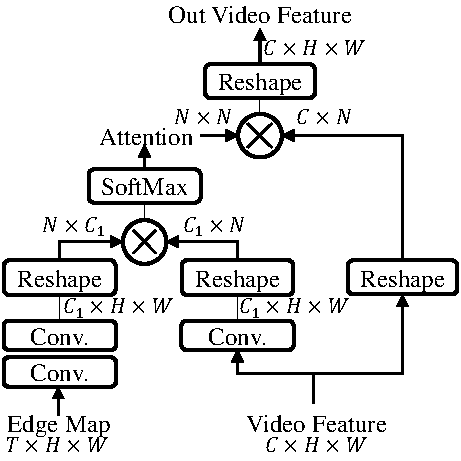
\includegraphics[width=0.7\columnwidth]{SEM} % Reduce the figure size so that it is slightly narrower than the column. Don't use precise values for figure width.This setup will avoid overfull boxes. 
	\caption{The architecture of SEM. The }
	\label{SEM}
\end{figure}




\subsection{Spatio-Temporal Inpainting (STI) Module}

With both inpained edges $\boldsymbol{E}$ and flow $\boldsymbol{O}$ for input frames, a spatio-temporal inpainting (STI) module is designed to obtain the final target frame $Y_t$.
%under the guidance of the  and motion tendency, which is helpful to the completion process of the target frame...
Notably, the inpained edge and flow can provide structural details and temporal information, respectively.
To generate realistic video content, STI adopts a coarse-to-fine architecture, consisting of a coarse network and a refinement network, as shown in Fig.~\ref{sti}.
First, the coarse network is implemented with 3D convolution to capture the temporal information, which targets to generate an initial rough completed frame.
Second, the refinement network is implemented with 2D convolution to enhance spatial details and refine the initial completed frame.

To make an adequate use of structural information in $\boldsymbol{E}$, an edge attention mechanism is designed for STI to generate structure-enhanced inaptining results.
As shown in Fig.~\ref{sti}, the edge attention mechanism first extracts the structure information from $\boldsymbol{E}$ via two separate convolution blocks.
Then, the extracted structure information will be interacted via out-product operation to capture high-level structure clues, such as object shape and spatial relationship.
Finally, the refined structure information will be encoded into the intermediate features of the input video via attention operation.
Furthermore, $\boldsymbol{E}$ serves as an auxiliary input, concatenated with $\boldsymbol{X}$ and $\boldsymbol{M}$, to STI.
After introducing structure information, the inpainted video content by STI becomes more structure-preserved and semantically realistic.

To smooth temporal flickers and aggregate complementary neighboring clues, the motion tendency information in $\boldsymbol{O}$ is utilized by warping the neighboring frames into the target frame and employing a frame reconstruction constraint.
Specifically, a flow warping loss is proposed:
\begin{equation}
\label{eq:inp_flow}
\mathcal{L}^I_{flo}=\sum_{\widehat{t}\in\mathcal{T}}\frac{1}{\left\|M^F_{\widehat{t}\Rightarrow t}\right\|_1}\left\| Y_t-\phi(O_{\widehat{t}\Rightarrow t},Y_{\widehat{t}}) \right\|_1,
\end{equation}
where $\mathcal{T}=\{t-7,t-3\}$. $\phi(O_{\widehat{t}\Rightarrow t},Y_{\widehat{t}})$ warps $Y_{\widehat{t}}$ to $Y_{t}$ using flow $O_{\widehat{t}\Rightarrow t}$.
Therefore, $\mathcal{L}^I_{flo}$ expects that all the neighboring frames can be well warped to the target frame with small reconstruction loss, rendering the inpainted frames to be temporal consistent.

%\(O_{t\Rightarrow t-3}\) is used to warp the inpainted $Y_{t-3}$ to aid the current $Y_{t}$, which provides a high temporal coherence.


%, which will generate a temporal smooth fine-detailed $Y_{t}$.
Finally, the loss function for STI is:
\begin{equation}
\label{eq:inpain_all}
\mathcal{L}_{inp}=\mathcal{L}^{I}_{rec}+\mathcal{L}^I_{adv}+\mathcal{L}^I_{flo},
\end{equation}
where $\mathcal{L}^{I}_{rec}$, $\mathcal{L}^I_{adv}$, and $\mathcal{L}^I_{flo}$ are respectively reconstruction loss, adversarial loss and flow warping loss.
Inspired by \cite{}, $\mathcal{L}^{I}_{rec}$ consists of three terms by:
\begin{equation}
\begin{aligned}
\mathcal{L}^{I}_{rec}=&\frac{1}{\left\|\boldsymbol{M} \right\|_1}\left\|(\boldsymbol{Y}^i-\widetilde{\boldsymbol{Y}})\odot \boldsymbol{M}\right\|_1 +\frac{1}{\left\|M_t \right\|_1}\left\|(Y_t-\widetilde{Y}_t)\odot M_t\right\|_1\\
&+\mathbb{E}[\sum_{j}\frac{1}{N_j}\left\|\boldsymbol{\psi}_j(\widetilde{Y}_t)-\boldsymbol{\psi}_j(Y_t)\right\|_1]\\
&+\mathbb{E}_j[\left\|G^{\boldsymbol{\psi}_j}(\widetilde{Y}_t)-G^{\boldsymbol{\psi}_j}(Y_t)\right\|_1],
\end{aligned}
\end{equation}
where the first term is pixel $l_1$ loss to evaluate generation quality. 
The second term is the perceptual loss \cite{gatys2015neural}, which compares the semantic contents between the generated frame and ground truth.

$\boldsymbol{\psi}_j$ denotes the activation maps of $j_{th}$ layer in a network.
$N_j$ is the number of elements in layer $\boldsymbol{\psi}_j$. We use layers $relu_{1\_1}$, $relu_{2\_1}$, $relu_{3\_1}$, $relu_{4\_1}$ and $relu_{5\_1}$ of the VGG-19 network pre-trained on the ImageNet dataset for this loss.
The third term is the style loss, designed to prevent "checkerboard" artifacts \cite{Sajjadi_2017_ICCV} caused by transpose convolution. $G^{\boldsymbol{\psi}_j}$ is the Gram matrix calculated by auto-correlation of $\boldsymbol{\psi}_j$. The layers are the same as that of perceptual loss.

%The adversarial loss is only for the final $Y_{t}$
$\mathcal{L}^I_{adv}$ is defined as:
\begin{equation}
\label{eq:inp_adver}
\mathcal{L}^I_{adv}=\min\limits_{N^I} \max \limits_{D^I} \mathbb{E}[logD^I(\widetilde{Y}_t)]+\mathbb{E}log[1-D^I(Y_{t})],
\end{equation}
where $D^I$ possesses the same architecture as that of $D^E$, except the input dimension.